\documentclass[tikz,border=10pt]{standalone}
\usepackage{tikz}
% \usepackage{amsmath}
\usetikzlibrary{arrows.meta}
\begin{document}
	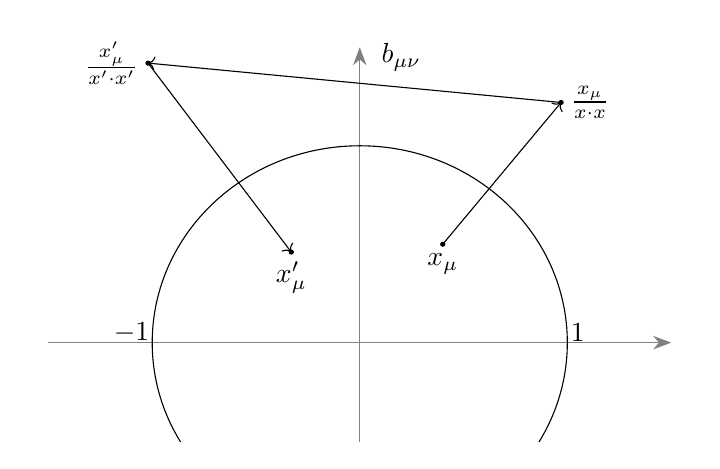
\begin{tikzpicture}[
 	         x                = 30,
	         scale            = 2.5,
	         axis/.style      = {help lines, -{Stealth[length = 1.5ex]}}]
	  \clip (-1.6,-0.5) rectangle (1.6,1.6);
	  \draw [axis] (-1.5,0) -- (1.5,0);
	  \draw [axis] (0,-1.5) -- (0,1.5);
	  \draw  (0,0) circle [radius=1,color=grey];
	  \filldraw [black] (0.4,0.5) circle [radius =0.01] node[anchor=north] {$x_{\mu}$};
	  \filldraw [black] (0.97,1.22) circle [radius =0.01] node[anchor=west] {$\frac{x_{\mu}}{x\cdot x}$};
	  \filldraw [black] (-1.02,1.42) circle [radius =0.01] node[anchor=east] {$\frac{x'_{\mu}}{x'\cdot x'}$};
	  \filldraw [black] (-0.33,0.46) circle [radius =0.01] node[anchor=north] {$x'_{\mu}$};
	  \draw [->] (0.4,0.5) -- (0.97,1.22);
	  \draw [->] (0.97,1.22) -- (-1.02,1.42) ;
	  \draw [->] (-1.02,1.42) -- (-0.33,0.46);
	  \draw (1.05,0.05) node {$1$};
	  \draw (-1.1,0.05) node {$-1$};
	  \draw (0.2,1.45)  node {$b_{\mu\nu}$};
	\end{tikzpicture}
\end{document}
